% Options for packages loaded elsewhere
\PassOptionsToPackage{unicode}{hyperref}
\PassOptionsToPackage{hyphens}{url}
%
\documentclass[
]{book}
\usepackage{amsmath,amssymb}
\usepackage{iftex}
\ifPDFTeX
  \usepackage[T1]{fontenc}
  \usepackage[utf8]{inputenc}
  \usepackage{textcomp} % provide euro and other symbols
\else % if luatex or xetex
  \usepackage{unicode-math} % this also loads fontspec
  \defaultfontfeatures{Scale=MatchLowercase}
  \defaultfontfeatures[\rmfamily]{Ligatures=TeX,Scale=1}
\fi
\usepackage{lmodern}
\ifPDFTeX\else
  % xetex/luatex font selection
\fi
% Use upquote if available, for straight quotes in verbatim environments
\IfFileExists{upquote.sty}{\usepackage{upquote}}{}
\IfFileExists{microtype.sty}{% use microtype if available
  \usepackage[]{microtype}
  \UseMicrotypeSet[protrusion]{basicmath} % disable protrusion for tt fonts
}{}
\makeatletter
\@ifundefined{KOMAClassName}{% if non-KOMA class
  \IfFileExists{parskip.sty}{%
    \usepackage{parskip}
  }{% else
    \setlength{\parindent}{0pt}
    \setlength{\parskip}{6pt plus 2pt minus 1pt}}
}{% if KOMA class
  \KOMAoptions{parskip=half}}
\makeatother
\usepackage{xcolor}
\usepackage{color}
\usepackage{fancyvrb}
\newcommand{\VerbBar}{|}
\newcommand{\VERB}{\Verb[commandchars=\\\{\}]}
\DefineVerbatimEnvironment{Highlighting}{Verbatim}{commandchars=\\\{\}}
% Add ',fontsize=\small' for more characters per line
\usepackage{framed}
\definecolor{shadecolor}{RGB}{248,248,248}
\newenvironment{Shaded}{\begin{snugshade}}{\end{snugshade}}
\newcommand{\AlertTok}[1]{\textcolor[rgb]{0.94,0.16,0.16}{#1}}
\newcommand{\AnnotationTok}[1]{\textcolor[rgb]{0.56,0.35,0.01}{\textbf{\textit{#1}}}}
\newcommand{\AttributeTok}[1]{\textcolor[rgb]{0.13,0.29,0.53}{#1}}
\newcommand{\BaseNTok}[1]{\textcolor[rgb]{0.00,0.00,0.81}{#1}}
\newcommand{\BuiltInTok}[1]{#1}
\newcommand{\CharTok}[1]{\textcolor[rgb]{0.31,0.60,0.02}{#1}}
\newcommand{\CommentTok}[1]{\textcolor[rgb]{0.56,0.35,0.01}{\textit{#1}}}
\newcommand{\CommentVarTok}[1]{\textcolor[rgb]{0.56,0.35,0.01}{\textbf{\textit{#1}}}}
\newcommand{\ConstantTok}[1]{\textcolor[rgb]{0.56,0.35,0.01}{#1}}
\newcommand{\ControlFlowTok}[1]{\textcolor[rgb]{0.13,0.29,0.53}{\textbf{#1}}}
\newcommand{\DataTypeTok}[1]{\textcolor[rgb]{0.13,0.29,0.53}{#1}}
\newcommand{\DecValTok}[1]{\textcolor[rgb]{0.00,0.00,0.81}{#1}}
\newcommand{\DocumentationTok}[1]{\textcolor[rgb]{0.56,0.35,0.01}{\textbf{\textit{#1}}}}
\newcommand{\ErrorTok}[1]{\textcolor[rgb]{0.64,0.00,0.00}{\textbf{#1}}}
\newcommand{\ExtensionTok}[1]{#1}
\newcommand{\FloatTok}[1]{\textcolor[rgb]{0.00,0.00,0.81}{#1}}
\newcommand{\FunctionTok}[1]{\textcolor[rgb]{0.13,0.29,0.53}{\textbf{#1}}}
\newcommand{\ImportTok}[1]{#1}
\newcommand{\InformationTok}[1]{\textcolor[rgb]{0.56,0.35,0.01}{\textbf{\textit{#1}}}}
\newcommand{\KeywordTok}[1]{\textcolor[rgb]{0.13,0.29,0.53}{\textbf{#1}}}
\newcommand{\NormalTok}[1]{#1}
\newcommand{\OperatorTok}[1]{\textcolor[rgb]{0.81,0.36,0.00}{\textbf{#1}}}
\newcommand{\OtherTok}[1]{\textcolor[rgb]{0.56,0.35,0.01}{#1}}
\newcommand{\PreprocessorTok}[1]{\textcolor[rgb]{0.56,0.35,0.01}{\textit{#1}}}
\newcommand{\RegionMarkerTok}[1]{#1}
\newcommand{\SpecialCharTok}[1]{\textcolor[rgb]{0.81,0.36,0.00}{\textbf{#1}}}
\newcommand{\SpecialStringTok}[1]{\textcolor[rgb]{0.31,0.60,0.02}{#1}}
\newcommand{\StringTok}[1]{\textcolor[rgb]{0.31,0.60,0.02}{#1}}
\newcommand{\VariableTok}[1]{\textcolor[rgb]{0.00,0.00,0.00}{#1}}
\newcommand{\VerbatimStringTok}[1]{\textcolor[rgb]{0.31,0.60,0.02}{#1}}
\newcommand{\WarningTok}[1]{\textcolor[rgb]{0.56,0.35,0.01}{\textbf{\textit{#1}}}}
\usepackage{longtable,booktabs,array}
\usepackage{calc} % for calculating minipage widths
% Correct order of tables after \paragraph or \subparagraph
\usepackage{etoolbox}
\makeatletter
\patchcmd\longtable{\par}{\if@noskipsec\mbox{}\fi\par}{}{}
\makeatother
% Allow footnotes in longtable head/foot
\IfFileExists{footnotehyper.sty}{\usepackage{footnotehyper}}{\usepackage{footnote}}
\makesavenoteenv{longtable}
\usepackage{graphicx}
\makeatletter
\def\maxwidth{\ifdim\Gin@nat@width>\linewidth\linewidth\else\Gin@nat@width\fi}
\def\maxheight{\ifdim\Gin@nat@height>\textheight\textheight\else\Gin@nat@height\fi}
\makeatother
% Scale images if necessary, so that they will not overflow the page
% margins by default, and it is still possible to overwrite the defaults
% using explicit options in \includegraphics[width, height, ...]{}
\setkeys{Gin}{width=\maxwidth,height=\maxheight,keepaspectratio}
% Set default figure placement to htbp
\makeatletter
\def\fps@figure{htbp}
\makeatother
\setlength{\emergencystretch}{3em} % prevent overfull lines
\providecommand{\tightlist}{%
  \setlength{\itemsep}{0pt}\setlength{\parskip}{0pt}}
\setcounter{secnumdepth}{5}
\usepackage{booktabs}
\ifLuaTeX
  \usepackage{selnolig}  % disable illegal ligatures
\fi
\usepackage[]{natbib}
\bibliographystyle{plainnat}
\IfFileExists{bookmark.sty}{\usepackage{bookmark}}{\usepackage{hyperref}}
\IfFileExists{xurl.sty}{\usepackage{xurl}}{} % add URL line breaks if available
\urlstyle{same}
\hypersetup{
  pdftitle={e-Campsis documentation},
  pdfauthor={Calvagone},
  hidelinks,
  pdfcreator={LaTeX via pandoc}}

\title{e-Campsis documentation}
\author{Calvagone}
\date{2023-11-20}

\usepackage{amsthm}
\newtheorem{theorem}{Theorem}[chapter]
\newtheorem{lemma}{Lemma}[chapter]
\newtheorem{corollary}{Corollary}[chapter]
\newtheorem{proposition}{Proposition}[chapter]
\newtheorem{conjecture}{Conjecture}[chapter]
\theoremstyle{definition}
\newtheorem{definition}{Definition}[chapter]
\theoremstyle{definition}
\newtheorem{example}{Example}[chapter]
\theoremstyle{definition}
\newtheorem{exercise}{Exercise}[chapter]
\theoremstyle{definition}
\newtheorem{hypothesis}{Hypothesis}[chapter]
\theoremstyle{remark}
\newtheorem*{remark}{Remark}
\newtheorem*{solution}{Solution}
\begin{document}
\maketitle

{
\setcounter{tocdepth}{1}
\tableofcontents
}
\hypertarget{about}{%
\chapter{About}\label{about}}

\href{https://ecampsis.shinyapps.io/free/}{e-Campsis} is a free web application developed by \href{https://www.calvagone.com/}{Calvagone} that provides an intuitive and user-friendly interface for setting up population PK/PD simulations.
The app is built on the R-package \href{https://calvagone.github.io/}{campsis}, which serves as a powerful frontend for running model-based simulations using \emph{mrgsolve} or \emph{rxode2}.

\hypertarget{e-campsis-versions}{%
\section{e-Campsis versions}\label{e-campsis-versions}}

\hypertarget{e-campsis-free}{%
\subsection{e-Campsis free}\label{e-campsis-free}}

\hypertarget{e-campsis-free-1}{%
\subsection{e-Campsis free+}\label{e-campsis-free-1}}

\emph{e-Campsis free} has certain limitations regarding the simulation size for unregistered users.

If you want to simulate up to 16 arms or scenarios, 100 subjects/arm and 250 observations/arm we invite you to become an authorized user of \emph{e-Campsis free+}.

Please send us the pre-filled email below and you will get an invitation to register as soon as possible: \href{mailto:campsis@calvagone.com}{\nolinkurl{campsis@calvagone.com}}

\hypertarget{e-campsis-pro}{%
\subsection{e-Campsis pro}\label{e-campsis-pro}}

At \textbf{Calvagone} we are currently working on an advanced version of e-Campsis including the following additional functionality:

\begin{itemize}
\tightlist
\item
  No limitation of number of subjects, observations, ODEs, arms or scenarios
\item
  Save all settings of your simulation project within the Shiny environment
\item
  Import external data into plots for visual comparison to simulations
\item
  Extensive library, including models with categorical endpoints
\item
  Sampling of covariates from external databases like e.g.~NHANES
\item
  Run trial replicates, taking into account parameter uncertainty
\item
  Post-processing of simulation results, applying for example NCA or statistical tests
\item
  Efficient generation of forest plots on derived simulation output (e.g.~Cmax, AUC, \href{mailto:effect@time}{\nolinkurl{effect@time}})
\item
  Semi-automatic parameter sensitivity analysis
\end{itemize}

For further information, contact us by clicking the link below: \href{mailto:campsis@calvagone.com}{\nolinkurl{campsis@calvagone.com}}

\hypertarget{application-interface}{%
\section{Application interface}\label{application-interface}}

The app consists of 4 main sections:

\begin{itemize}
\tightlist
\item
  \textbf{Model}: a powerful model editor to edit your Campsis model online. Try out one of the numerous models available from the library and adapt it to your needs.
\item
  \textbf{Trial design}: an easy-to-use interface to quickly set-up the dosing regimen, observation times and covariates.
\item
  \textbf{Simulation}: a single screen dedicated to the simulation configuration and visualisation of the results. Explore different scenarios of parameter settings quickly and interactively.
\item
  \textbf{Download}: last but not least, download the model, parameters and the whole code of the simulation to reproduce what you see in the app on your computer using the open-source package campsis.
\end{itemize}

\hypertarget{model-tab}{%
\chapter{Model tab}\label{model-tab}}

\begin{figure}
\centering
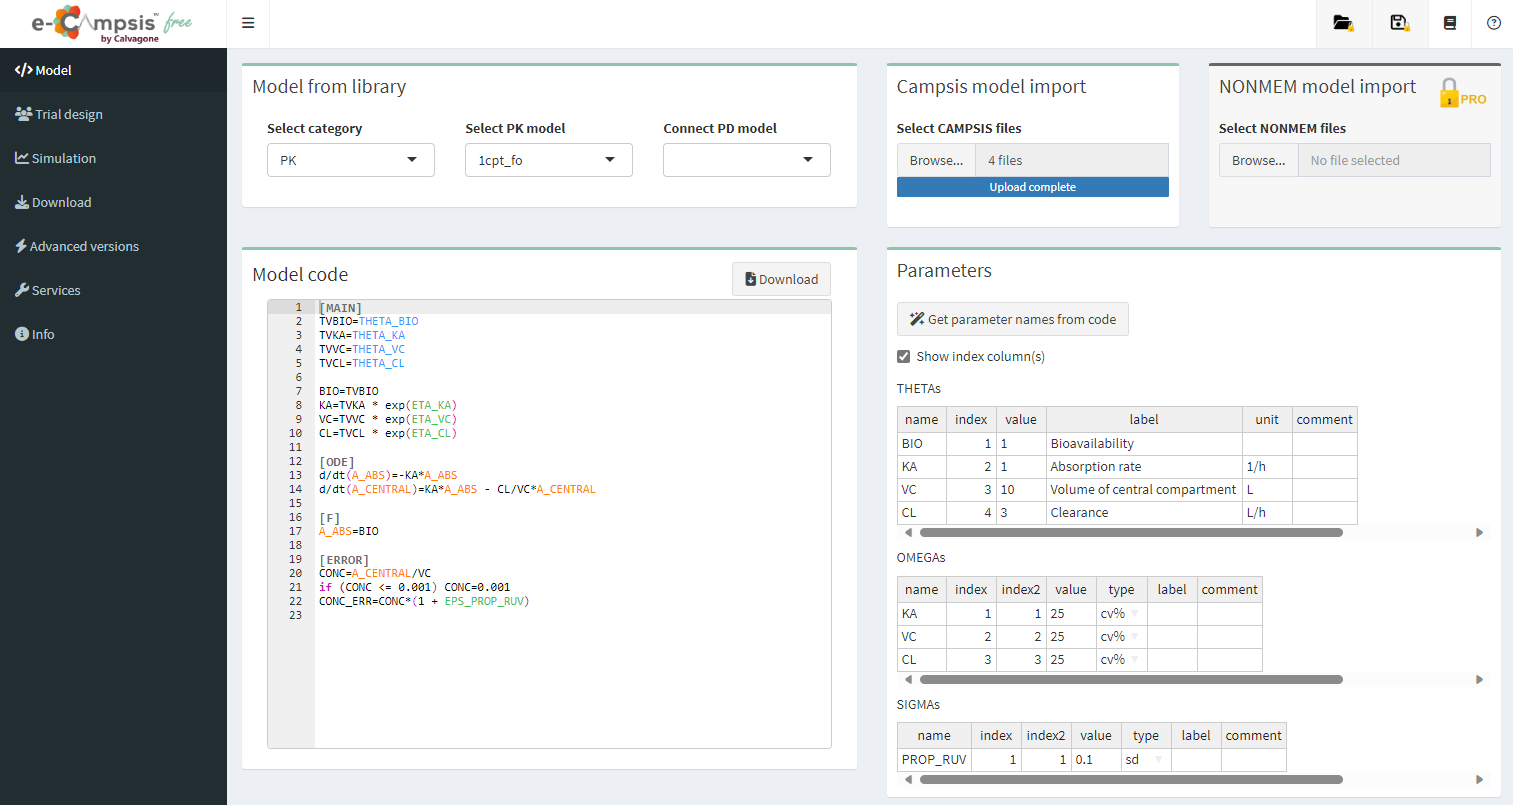
\includegraphics{ecampsis_model_tab.png}
\caption{e-Campis Model tab}
\end{figure}

\hypertarget{model-from-library}{%
\section{Model from library}\label{model-from-library}}

When entering the app, a simple PK model is already loaded by default.

A different PK model can be selected from a large library (``Select PK model''), or a PD model can be connected (``Connect PD model'') to the PK model. In ``Select category'', NONMEM models or TMDD models can be also loaded.

\hypertarget{campsis-model-import}{%
\section{Campsis model import}\label{campsis-model-import}}

An existing Campsis model can be uploaded from this box (including files \emph{model.campsis}, \emph{omega.csv}, \emph{theta.csv} and \emph{sigma.csv}).

\hypertarget{nonmem-model-import}{%
\section{NONMEM model import}\label{nonmem-model-import}}

In the pro version, an existing NONMEM model can be uploaded from this box (including files \emph{.mod} and \emph{.ext}).

The NONMEM import functionality will be installed, the process can take several minutes. A notification will popup when done.

\hypertarget{model-code}{%
\section{Model code}\label{model-code}}

The model code is shown in the editor window where it can be easily modified. Please note that the code is case sensitive (e.g.~\emph{log}, \emph{exp}, \emph{sqrt} should be used). The power function is \emph{pow(x,d)}, \emph{x} to the power of \emph{d}.

\hypertarget{parameters}{%
\section{Parameters}\label{parameters}}

The list of parameters for THETA, OMEGA and SIGMA is given in this box. Their values and labels can be changed. Comments can be added.

The type for OMEGA and SIGMA can be changed: sd, var, covar, cv, cv\%, cor, for standard deviation, variance, covariance, coefficient of variation, coefficient of variation (as \%) or correlation, respectively.

Correlations between omegas can be added by right-clicking on a cell in the OMEGA table. For example, enter ``KA, VC'' as name, 1 and 2 in index and index2, and add the correlation value.

Clicking on ``Get parameter names from code'', the code will be scanned for the \#THETA, \#OMEGA and \#SIGMA and the names will be extracted and added to the table.

\hypertarget{trial-design}{%
\chapter{Trial design}\label{trial-design}}

\hypertarget{trial-design-1}{%
\section{Trial design}\label{trial-design-1}}

Several study arms can be configured.

For each arm tab, the following information can be entered:

\begin{itemize}
\tightlist
\item
  Number of subjects
\item
  Arm label
\item
  Administration type
\item
  Dose amount
\item
  Compartment (in which compartment the dose should be assigned)
\item
  Dosing interval
\item
  Add. doses (number of additional doses)
\item
  Observations (observation time), to be written in R format, e.g.~\emph{seq(0,24,by=1)} or \emph{c(seq(0, 5), seq(0, 5)+168, seq(0,5)+336, seq(0,504,6))}. Enable the ``as-time-after-dose'' box, if you want to replicate the observation schedule after each dose.
\item
  Covariates; e.g.~\emph{BW=70}, \emph{DOSE=1\textbar BW=70}, \emph{WT=NormalDistribution(mean=70, sd=10)}
\item
  Dose adaptation formula (useful if the dose has to be adapted to the body weight); e.g.~\_DOSE*BW\_
\end{itemize}

\hypertarget{summary}{%
\section{Summary}\label{summary}}

A summary of your trial design in shown in this box, where you can quickly visualise the characteristics of your arms.

\hypertarget{custom-dataset}{%
\section{Custom dataset}\label{custom-dataset}}

The simulation dataset (arms) can be further edited by clicking ``Edit dataset'' button.

\href{https://calvagone.github.io/campsis.doc/articles/v01_dataset.html}{See the Campsis help}

\hypertarget{simulation}{%
\chapter{Simulation}\label{simulation}}

Once your trial design is configured, go to the Simulation Tab and the simulation is instantaneously executed.

\hypertarget{footnotes-and-citations}{%
\chapter{Footnotes and citations}\label{footnotes-and-citations}}

\hypertarget{footnotes}{%
\section{Footnotes}\label{footnotes}}

Footnotes are put inside the square brackets after a caret \texttt{\^{}{[}{]}}. Like this one \footnote{This is a footnote.}.

\hypertarget{citations}{%
\section{Citations}\label{citations}}

Reference items in your bibliography file(s) using \texttt{@key}.

For example, we are using the \textbf{bookdown} package \citep{R-bookdown} (check out the last code chunk in index.Rmd to see how this citation key was added) in this sample book, which was built on top of R Markdown and \textbf{knitr} \citep{xie2015} (this citation was added manually in an external file book.bib).
Note that the \texttt{.bib} files need to be listed in the index.Rmd with the YAML \texttt{bibliography} key.

The RStudio Visual Markdown Editor can also make it easier to insert citations: \url{https://rstudio.github.io/visual-markdown-editing/\#/citations}

\hypertarget{blocks}{%
\chapter{Blocks}\label{blocks}}

\hypertarget{equations}{%
\section{Equations}\label{equations}}

Here is an equation.

\begin{equation} 
  f\left(k\right) = \binom{n}{k} p^k\left(1-p\right)^{n-k}
  \label{eq:binom}
\end{equation}

You may refer to using \texttt{\textbackslash{}@ref(eq:binom)}, like see Equation \eqref{eq:binom}.

\hypertarget{theorems-and-proofs}{%
\section{Theorems and proofs}\label{theorems-and-proofs}}

Labeled theorems can be referenced in text using \texttt{\textbackslash{}@ref(thm:tri)}, for example, check out this smart theorem \ref{thm:tri}.

\begin{theorem}
\protect\hypertarget{thm:tri}{}\label{thm:tri}For a right triangle, if \(c\) denotes the \emph{length} of the hypotenuse
and \(a\) and \(b\) denote the lengths of the \textbf{other} two sides, we have
\[a^2 + b^2 = c^2\]
\end{theorem}

Read more here \url{https://bookdown.org/yihui/bookdown/markdown-extensions-by-bookdown.html}.

\hypertarget{callout-blocks}{%
\section{Callout blocks}\label{callout-blocks}}

The R Markdown Cookbook provides more help on how to use custom blocks to design your own callouts: \url{https://bookdown.org/yihui/rmarkdown-cookbook/custom-blocks.html}

\hypertarget{sharing-your-book}{%
\chapter{Sharing your book}\label{sharing-your-book}}

\hypertarget{publishing}{%
\section{Publishing}\label{publishing}}

HTML books can be published online, see: \url{https://bookdown.org/yihui/bookdown/publishing.html}

\hypertarget{pages}{%
\section{404 pages}\label{pages}}

By default, users will be directed to a 404 page if they try to access a webpage that cannot be found. If you'd like to customize your 404 page instead of using the default, you may add either a \texttt{\_404.Rmd} or \texttt{\_404.md} file to your project root and use code and/or Markdown syntax.

\hypertarget{metadata-for-sharing}{%
\section{Metadata for sharing}\label{metadata-for-sharing}}

Bookdown HTML books will provide HTML metadata for social sharing on platforms like Twitter, Facebook, and LinkedIn, using information you provide in the \texttt{index.Rmd} YAML. To setup, set the \texttt{url} for your book and the path to your \texttt{cover-image} file. Your book's \texttt{title} and \texttt{description} are also used.

This \texttt{gitbook} uses the same social sharing data across all chapters in your book- all links shared will look the same.

Specify your book's source repository on GitHub using the \texttt{edit} key under the configuration options in the \texttt{\_output.yml} file, which allows users to suggest an edit by linking to a chapter's source file.

Read more about the features of this output format here:

\url{https://pkgs.rstudio.com/bookdown/reference/gitbook.html}

Or use:

\begin{Shaded}
\begin{Highlighting}[]
\NormalTok{?bookdown}\SpecialCharTok{::}\NormalTok{gitbook}
\end{Highlighting}
\end{Shaded}


  \bibliography{book.bib,packages.bib}

\end{document}
